\chapter{Analisis de requisitos}\label{requisitos}

\section{Actores del sistema}

El sistema define cuatro actores principales:

\begin{itemize}
	\item \textbf{Consumidor:} crea listas, compara precios, optimiza rutas, usa OCR
		y consulta al asistente.
	\item \textbf{Comercio/PYME:} gestiona precios y promociones desde el portal business.
	\item \textbf{Administrador:} verifica perfiles, modera datos y supervisa operacion.
	\item \textbf{Sistema automatizado:} tareas de scraping y mantenimiento en segundo plano.
\end{itemize}

\section{Requisitos de informacion}

El modelo de informacion se articula en doce bloques (RI-001 a RI-012), que cubren:

\begin{itemize}
	\item usuarios y preferencias de optimizacion,
	\item catalogo (productos, categorias, marcas),
	\item tiendas geolocalizadas y cadenas,
	\item precios actuales e historicos,
	\item listas de compra y resultados de optimizacion,
	\item perfiles business y promociones,
	\item sesiones OCR y conversaciones del asistente.
\end{itemize}

\section{Requisitos funcionales}

Se definieron 35 requisitos funcionales (RF-001 a RF-035) agrupados por dominios:

\begin{table}[h]
\centering
\caption{Agrupacion de requisitos funcionales}
\label{tab:rf-grupos}
\begin{tabular}{|l|c|l|}
\hline
\textbf{Dominio} & \textbf{IDs} & \textbf{Capacidad principal} \\
\hline
Autenticacion y perfil & RF-001..RF-005 & Registro, login JWT, preferencias \\
Catalogo de productos & RF-006..RF-010 & Busqueda, detalle, crowdsourcing \\
Tiendas y mapa & RF-011..RF-014 & Proximidad, detalle, favoritos \\
Precios & RF-015..RF-019 & Comparacion, historico, alertas \\
Listas de compra & RF-020..RF-023 & CRUD, compartir, plantillas \\
Optimizador & RF-024..RF-027 & Ruta multicriterio y recalculo \\
OCR & RF-028..RF-029 & Captura y matching fuzzy \\
Asistente LLM & RF-030..RF-031 & Consultas naturales y sugerencias \\
Portal business & RF-032..RF-034 & Onboarding, precios, promociones \\
Notificaciones & RF-035 & Push/email por eventos \\
\hline
\end{tabular}
\end{table}

\section{Criterios de aceptacion del producto}

Los criterios de aceptacion se validan a nivel funcional y de experiencia:

\begin{itemize}
	\item flujo de alta y acceso operativo en menos de 3 minutos,
	\item comparacion de cesta completa en entorno de tiendas cercanas,
	\item optimizacion con top-3 rutas y desglose por parada,
	\item OCR con confirmacion/edicion previa a insercion en lista,
	\item portal PYME con gestion de precios y promociones,
	\item notificaciones de eventos criticos (alertas, promociones, cambios compartidos).
\end{itemize}

\section{Requisitos no funcionales}

Se definieron ocho requisitos no funcionales (RNF-001 a RNF-008):

\begin{itemize}
	\item rendimiento API (p95 bajo para operaciones CRUD y optimizacion),
	\item disponibilidad de staging,
	\item seguridad (JWT, HTTPS, rate limiting),
	\item usabilidad (flujo principal corto y criterios de accesibilidad),
	\item escalabilidad arquitectonica,
	\item mantenibilidad con cobertura y convenciones,
	\item compatibilidad multiplataforma,
	\item cumplimiento RGPD.
\end{itemize}

\section{Reglas de negocio}

Las reglas RN-001..RN-010 gobiernan limites y politicas operativas:

\begin{itemize}
	\item radio maximo de busqueda y numero maximo de paradas,
	\item caducidad y prioridad de fuentes de precio,
	\item restricciones del asistente a dominio de compra,
	\item verificacion previa de perfiles business,
	\item politicas de scraping responsable y frecuencia de ejecucion.
\end{itemize}

\section{Diagramas de casos de uso}

Los diagramas de casos de uso recogen las interacciones principales de cada actor con el sistema.

\begin{figure}[htbp]
\centering
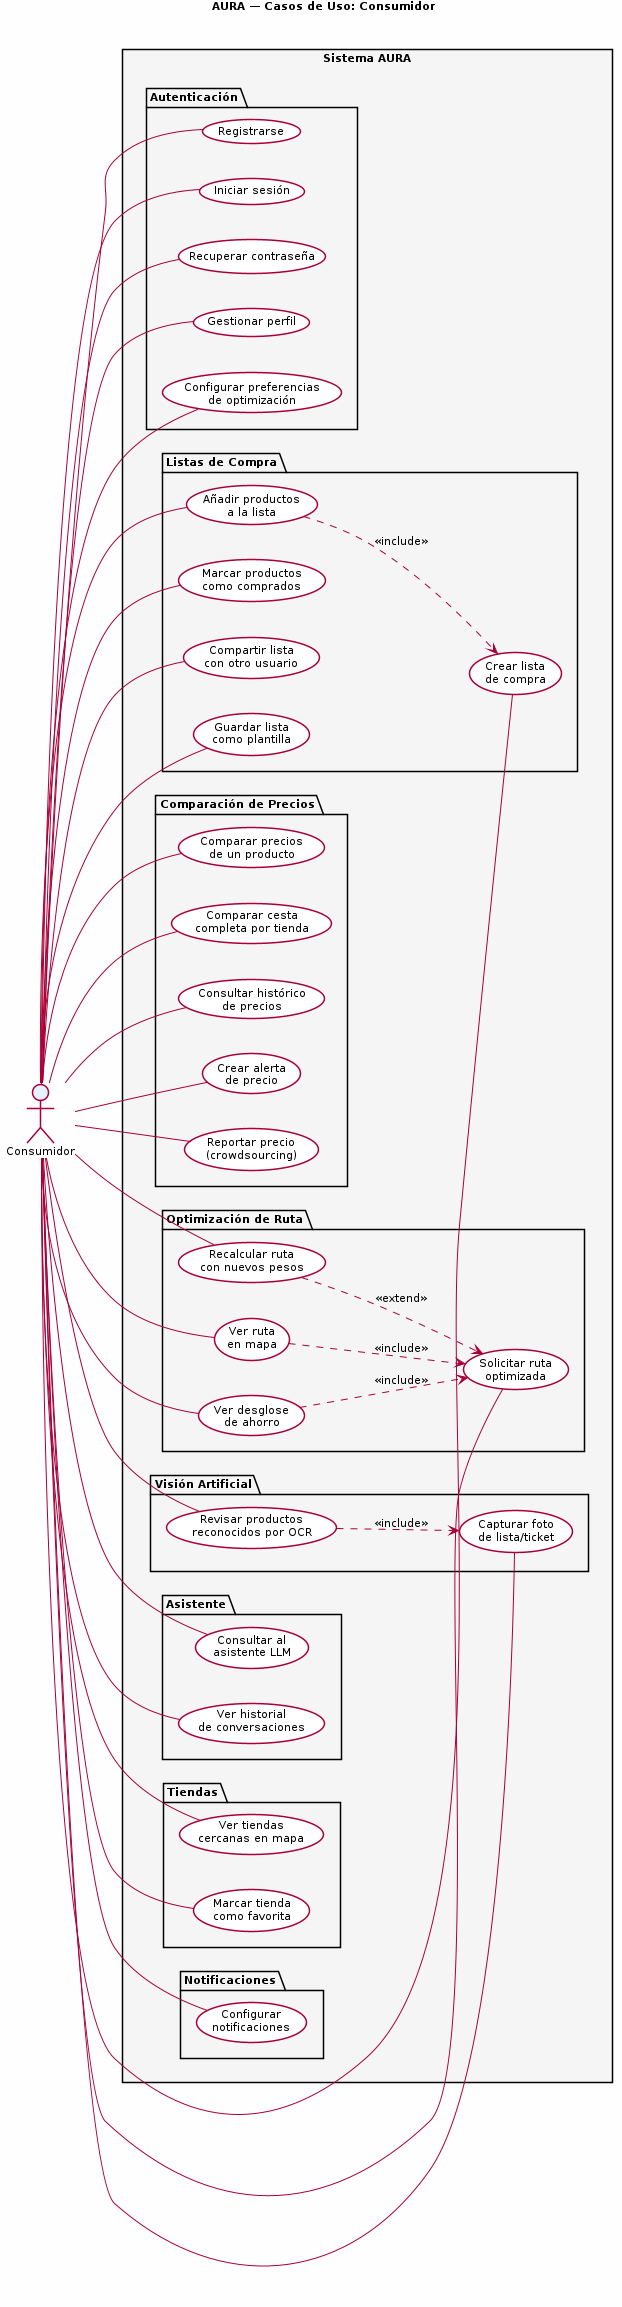
\includegraphics[width=0.85\textwidth]{../diagramas/casos-uso/casos-uso-consumidor.png}
\caption{Casos de uso del Consumidor}
\label{fig:casos-uso-consumidor}
\end{figure}

\begin{figure}[htbp]
\centering
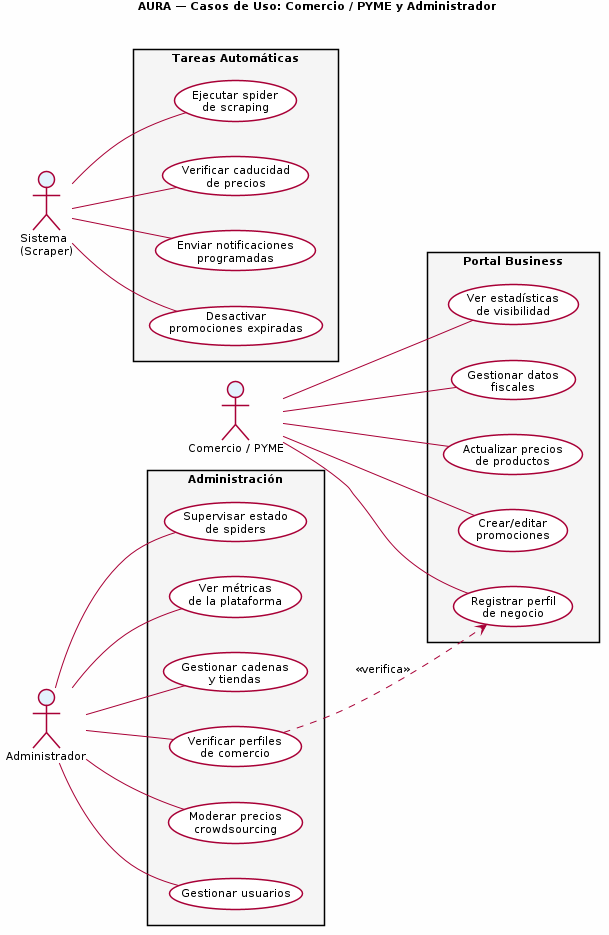
\includegraphics[width=0.85\textwidth]{../diagramas/casos-uso/casos-uso-comercio-admin.png}
\caption{Casos de uso del Comercio y Administrador}
\label{fig:casos-uso-comercio}
\end{figure}

\section{Trazabilidad}

La trazabilidad entre requisitos, implementacion y pruebas se mantiene en:

\begin{itemize}
	\item \texttt{docs/memoria/07-requisitos.md} (especificacion completa),
	\item \texttt{TASKS.md} (estado por fase/tarea),
	\item \texttt{tests/unit}, \texttt{tests/integration} y \texttt{frontend/web/e2e}
		(verificacion ejecutable).
\end{itemize}
